% Provenance (never printed): see sources/outline_sources.md (Year 1: compaction and
% cementation; basin types; subsidence, accommodation and sea-level change). Exercise and
% problem values in the Book 3 scratch calculator calc/ch23.py; figure data from
% figdata/bachelor-1/compaction.py and sea_level.py.
% Porosity and permeability are Book 1's (g6); diagenesis was met in Book 2 (g12) and is
% re-founded here; sedimentary basin was met in Book 2 (g11) and is re-founded here;
% isostasy and the equal-mass proposition are ch. 11's; passive margins and rifts ch. 13's;
% effective stress ch. 16's; the Last Glacial Maximum and glacial cycles Book 2's (g12).
% Pressure solution is defined in the Year 3 volume (deformation mechanisms): prose only.
% Backstripping, the stretching model and the comparison of basins are the Year 2 volume's.
\chapter{Diagenese en sedimentaire bekkens}\label{ch:b1:diagenesis-basins}

Strandzand is los: de helft ervan, naar volume, is water tussen de korrels. Drie kilometer diep begraven komt hetzelfde zand als hard zandsteen weer omhoog in een boorkern, zijn korrels samengedrukt en de ruimte ertussen sterk verkleind en deels gevuld met nieuw kwarts. Tussen het strand en de kern liggen miljoenen jaren waarin het sediment werd begraven onder meer sediment, samengeperst, verhit en doordrenkt met water dat sommige mineralen oploste en andere afzette. Dit hoofdstuk volgt die veranderingen, en keert dan terug naar de plaatsen waar sediment kilometers dik kan ophopen --- de sedimentaire bekkens --- en naar de twee dingen die daar ruimte maken: het zinken van de vloer, en het stijgen en dalen van de zee.

\begin{recall}
De porositeit van een gesteente is de fractie van zijn volume die uit poriën bestaat, en zijn permeabiliteit meet hoe gemakkelijk water erdoor stroomt (Boek~1, klas~6). Een gebied is in \omterm{def:b1:isostasy-gravity:isostasy}{isostasie} wanneer elke kolom tot aan de \omterm{def:b1:isostasy-gravity:isostasy}{compensatiediepte} dezelfde massa bevat (\cref{prop:b1:isostasy-gravity:equal-mass}). Riften openen door normale breuken, en passieve marges zijn de randen van continenten die achterblijven wanneer een rift een oceaan wordt (\cref{ch:b1:rifts-ridges-margins}). De \omterm{def:b1:stress-strain-rheology:lithostatic}{effectieve spanning} is de spanning minus de druk van de poriënvloeistof (\cref{def:b1:stress-strain-rheology:lithostatic}). De laatste glaciale cyclus bereikte zijn Laatste Glaciaal Maximum ongeveer twintig duizend jaar geleden (Boek~2, klas~12). Zandsteen, schalie en hun milieus zijn die van \cref{ch:b1:clastic-sediments}; kalksteen, krijt, dolomiet en \omterm{def:b1:chemical-biogenic-sediments:evaporite}{verdampingsgesteenten} die van \cref{ch:b1:chemical-biogenic-sediments}.
\end{recall}

\section{Compactie}\label{sec:b1:diagenesis-basins:compaction}

Een pas afgezet sediment is een losse stapeling van korrels met water ertussen. Alles wat er daarna gebeurt, na de afzetting en vóór metamorfose, terwijl het bij de lage temperaturen en drukken van de bovenste paar kilometers van de \omterm{def:b1:layered-earth:layers}{korst} blijft, behoort tot één familie van processen.

\begin{definition}[Diagenese]\label{def:b1:diagenesis-basins:diagenesis}
\emph{Diagenese}\index{diagenese} is de verzameling fysische, chemische en biologische veranderingen die een sediment ondergaat na zijn afzetting, bij de temperaturen en drukken van de bovenste \omterm{def:b1:layered-earth:layers}{korst}, lager dan die van metamorfose. Zij omvat \omterm{def:b1:diagenesis-basins:compaction}{compactie}, \omterm{def:b1:diagenesis-basins:cement}{cementatie}, de oplossing van korrels en de vervanging van het ene \omterm{def:b1:rock-forming-minerals:mineral}{mineraal} door het andere; samen maken zij van een los sediment een sedimentair gesteente.
\end{definition}

De eerste van deze veranderingen is mechanisch. Elke nieuwe laag voegt zijn gewicht toe aan die eronder. De korrels worden samengedrukt, schuiven en draaien tot een dichtere stapeling, de zachte (kleiplaatjes, gesteentefragmenten, \omterm{def:b1:rock-forming-minerals:groups}{mica}) buigen tussen de harde, en het water ertussen wordt uitgedreven.
% ledger: og:diagenesis

\begin{definition}[Compactie, decompactie]\label{def:b1:diagenesis-basins:compaction}
\emph{Compactie}\index{compactie} is het volumeverlies van een sediment onder het gewicht van de sedimenten erboven, door de dichtere stapeling van zijn korrels, het uitdrijven van zijn poriënwater en, dieper, de oplossing van korrels waar zij elkaar raken. \emph{Decompactie}\index{decompactie} is de berekening die een begraven laag terugbrengt tot de dikte die zij had bij een eerdere, ondiepere begraving, meestal aan het oppervlak, toen zij werd afgezet.
\end{definition}

Porositeiten die in boorputten zijn gemeten, dalen met de diepte, steil nabij het oppervlak en daarna steeds trager. In 1930 paste L.~F. Athy er een exponentiële functie op aan, en die aanpassing is sindsdien het uitgangspunt van compactiestudies gebleven.
% ledger: sc80:athy

\begin{proposition}[De wet van Athy]\label{prop:b1:diagenesis-basins:athy}
In een stapel sediment van één lithologie, gecompacteerd onder zijn eigen gewicht met zijn poriënwater vrij om te ontsnappen, is de porositeit op de diepte $z$ onder het oppervlak
\[
  \varphi(z) = \varphi_0\, e^{-z/\lambda},
\]
waarin $\varphi_0$, de oppervlakteporositeit, en $\lambda$, de vervalslengte, van de lithologie afhangen. Dit is de \emph{wet van Athy}\index{wet van Athy}.
\end{proposition}
\admitted

De wet is een empirische fit, geen gevolg van de theorie. Haar parameters worden lithologie voor lithologie gemeten uit de porositeiten van putten; de waarden van \cref{tab:b1:diagenesis-basins:athy}, gepubliceerd in een studie van de \omterm{def:b1:diagenesis-basins:subsidence}{subsidentie} van de Noordzee, worden veel gebruikt om voor \omterm{def:b1:diagenesis-basins:compaction}{compactie} te corrigeren. Schalie begint met meer water dan zand maar verliest het over een kortere afstand; krijt, aan het oppervlak de poreusste van de drie, verliest het het snelst van alle. Op \qty{3000}{m} geeft de wet een porositeit van \num{0.22} voor zandsteen, \num{0.14} voor schalie en \num{0.08} voor krijt (figuur hieronder): het strandzand van het begin van dit hoofdstuk heeft meer dan de helft van zijn poriën verloren.
% ledger: pybacktrack:compaction, sc80:north-sea

\begin{table}[htbp]
\centering
\begin{tabular}{lccc}
\hline
lithologie & oppervlakteporositeit $\varphi_0$ & vervalslengte $\lambda$ (m) & korreldichtheid (\unit{kg.m^{-3}}) \\
\hline
schalie            & 0.63 & 1960 & 2700 \\
zandsteen          & 0.49 & 3704 & 2650 \\
kleiige zandsteen  & 0.56 & 2564 & 2680 \\
krijt              & 0.70 & 1408 & 2710 \\
\hline
\end{tabular}
\caption{De parameters van de \omterm{prop:b1:diagenesis-basins:athy}{wet van Athy} en de dichtheden van de korrels voor vier lithologieën, naar Sclater en Christie (1980), zoals opgenomen in de open backtrackingsoftware pyBacktrack.}
\label{tab:b1:diagenesis-basins:athy}
\end{table}
% ledger: pybacktrack:compaction

\omterm{def:b1:diagenesis-basins:compaction}{Compactie} perst water uit; zij voegt geen korrels toe en neemt ze ook niet weg, zolang niets wordt opgelost en afgevoerd of als \omterm{def:b1:diagenesis-basins:cement}{cement} wordt aangevoerd. Het volume van de korrels in een kolom is daarom de grootheid die men moet volgen terwijl de kolom wordt begraven.

\begin{proposition}[Vaste dikte van een laag]\label{prop:b1:diagenesis-basins:solid}
Onder de \omterm{prop:b1:diagenesis-basins:athy}{wet van Athy} bevat een laag tussen de dieptes $z_1 < z_2$ per oppervlakte-eenheid een
volume korrels dat gelijk is aan de dikte
\[
  s = (z_2 - z_1) - \varphi_0 \lambda \left( e^{-z_1/\lambda} - e^{-z_2/\lambda} \right).
\]
Als de laag zonder verlies of winst van korrels naar een nieuwe diepte wordt verplaatst, voldoen haar nieuwe top
$z_1'$ en onderkant $z_2'$ aan $s(z_1', z_2') = s(z_1, z_2)$, en voor een gegeven
$z_1'$ heeft deze vergelijking precies één oplossing $z_2'$.
\end{proposition}

\begin{proof}
Een plak van dikte $\mathrm dz$ op de diepte $z$ bevat het volume korrels
$(1 - \varphi(z))\,\mathrm dz$ per oppervlakte-eenheid. Geïntegreerd van $z_1$ tot $z_2$,
\[
  s = \int_{z_1}^{z_2} \bigl(1 - \varphi_0 e^{-z/\lambda}\bigr)\,\mathrm dz
    = (z_2 - z_1) - \varphi_0\lambda\left(e^{-z_1/\lambda} - e^{-z_2/\lambda}\right).
\]
Met de top vast op $z_1'$ heeft de functie $f(b) = s(z_1', b)$ de
afgeleide $1 - \varphi(b) > 0$, omdat een porositeit kleiner dan één is; zij is
continu, nul bij $b = z_1'$ en groeit zonder grens, dus neemt zij de waarde
$s(z_1, z_2)$ precies één keer aan.
\end{proof}

\begin{method}[Een laag decompacteren]\label{met:b1:diagenesis-basins:decompaction}
\begin{enumerate}
  \item Lees de top $z_1$ en de onderkant $z_2$ van de laag vandaag af, en haar parameters $\varphi_0$ en $\lambda$
        (\cref{tab:b1:diagenesis-basins:athy}).
  \item Bereken haar vaste dikte $s$ met
        \cref{prop:b1:diagenesis-basins:solid}.
  \item Kies de diepte $z_1'$ van haar top op het eerdere tijdstip --- nul om haar tot het oppervlak te herstellen.
  \item Los $s(z_1', b) = s$ op naar de nieuwe onderkant $b$ met de methode van Newton: begin met $b_0 = z_1' + (z_2 - z_1)$ en herhaal
        \[
          b_{k+1} = b_k - \frac{s(z_1', b_k) - s}{1 - \varphi(b_k)}
        \]
        tot de verandering onder de gewenste precisie ligt; twee of drie stappen volstaan meestal.
  \item De dikte van de laag op dat tijdstip is $b - z_1'$; haar gemiddelde
        porositeit is $1 - s/(b - z_1')$.
\end{enumerate}
\end{method}

Neem \qty{500}{m} schalie tussen \qty{3000}{m} en \qty{3500}{m}. Zij bevat \qty{440}{m} korrels en slechts \qty{60}{m} water, een gemiddelde porositeit van \num{0.12}. Teruggebracht naar het oppervlak maken dezelfde korrels een laag van \qty{891}{m} dik, waarvan de helft water is (figuur hieronder). De dikte van een begraven schalie is nauwelijks meer dan de helft van wat werd afgezet; sedimentatiesnelheden die uit begraven secties worden gelezen, moeten worden gedecompacteerd voordat zij worden vergeleken met snelheden die vandaag worden gemeten.
% computed in figdata/bachelor-1/compaction.py; ledger: pybacktrack:compaction

\begin{omfigure}
\begin{tikzpicture}[font=\footnotesize]
\begin{axis}[name=phi, width=7.6cm, height=7.2cm, xmin=0, xmax=0.75, ymin=0, ymax=5000,
    y dir=reverse, xlabel={porositeit $\varphi$}, ylabel={diepte (m)},
    xtick={0,0.2,0.4,0.6}, ytick={0,1000,...,5000},
    legend style={at={(0.97,0.03)}, anchor=south east, font=\scriptsize, draw=none, fill=white, fill opacity=0.85, text opacity=1},
    legend cell align=left]
  \addplot[thick, omLithSand!50!black] table[x=phi_sand, y=z] {figdata/out/bachelor-1-compaction-curves.dat};
  \addplot[thick, omThm, densely dashed] table[x=phi_shale, y=z] {figdata/out/bachelor-1-compaction-curves.dat};
  \addplot[thick, omLithLime!50!black, dash dot] table[x=phi_chalk, y=z] {figdata/out/bachelor-1-compaction-curves.dat};
  \legend{zandsteen, schalie, krijt}
  \draw[black!50, dotted] (axis cs:0,3000) -- (axis cs:0.75,3000);
\end{axis}
\begin{axis}[at={(phi.east)}, anchor=west, xshift=1.6cm, width=6.4cm, height=7.2cm,
    ybar stacked, bar width=1.1cm, ymin=0, ymax=1000, enlarge x limits=0.45,
    symbolic x coords={buried, surface}, xtick=data,
    xticklabels={{op 3000--3500 m}, {aan het oppervlak}},
    ylabel={dikte van de laag (m)}, ytick={0,200,...,1000},
    legend style={at={(0.03,0.97)}, anchor=north west, font=\scriptsize, draw=none},
    legend cell align=left]
  \addplot[fill=omLithShale, draw=black!60] table[x=state, y=solid] {figdata/out/bachelor-1-compaction-demo.dat};
  \addplot[fill=omSea, draw=black!60] table[x=state, y=pore] {figdata/out/bachelor-1-compaction-demo.dat};
  \legend{korrels, poriënwater}
  \node[anchor=south] at (axis cs:buried,500) {\qty{500}{m}};
  \node[anchor=south] at (axis cs:surface,891) {\qty{891}{m}};
\end{axis}
\end{tikzpicture}

{\small Links: porositeit tegen diepte volgens de \omterm{prop:b1:diagenesis-basins:athy}{wet van Athy} voor zandsteen, schalie en krijt, met de parameters van \cref{tab:b1:diagenesis-basins:athy}. Rechts: \qty{500}{m} schalie tussen \qty{3000}{m} en \qty{3500}{m}, en dezelfde laag gedecompacteerd tot het oppervlak: de korrels (\qty{440}{m}) blijven behouden, het water niet.}
\label{fig:b1:diagenesis-basins:compaction}
\end{omfigure}
% computed in figdata/bachelor-1/compaction.py; ledger: pybacktrack:compaction

De \omterm{prop:b1:diagenesis-basins:athy}{wet van Athy} geldt alleen zolang het water kan vertrekken. \omterm{def:b1:diagenesis-basins:compaction}{Compactie} wordt gedreven door de \omterm{def:b1:stress-strain-rheology:lithostatic}{effectieve spanning}, het gewicht van het gesteente erboven minus de druk van het water in de poriën (\cref{ch:b1:stress-strain-rheology}). Waar een dikke schalie sneller wordt begraven dan haar water kan wegsijpelen, draagt het water een deel van de belasting, stijgt de poriëndruk boven de hydrostatische, en houdt de schalie een porositeit die te hoog is voor haar diepte: zij is overgedrukt, en de correctie voor \omterm{def:b1:diagenesis-basins:compaction}{compactie} moet daarmee rekening houden.
% ledger: sc80:north-sea

Dieper wordt \omterm{def:b1:diagenesis-basins:compaction}{compactie} chemisch. Waar twee kwartskorrels op elkaar drukken door een film van water, en vooral waar een vlokje klei of \omterm{def:b1:rock-forming-minerals:groups}{mica} ertussen ligt, lost kwarts op bij het contact; het silica diffundeert een korte weg door het water en wordt opnieuw afgezet op schone kwartsoppervlakken die naar de open poriën gericht zijn. De korrels dringen in elkaar door, en oplossing die zich langs oppervlakken concentreert, laat stylolieten achter, gezaagde naden van het onoplosbare residu. Deze drukoplossing, die Boek~5 als een deformatiemechanisme behandelt, is zowel de laatste fase van \omterm{def:b1:diagenesis-basins:compaction}{compactie} als de bron van het gewoonste \omterm{def:b1:diagenesis-basins:cement}{cement} van zandsteen.
% ledger: walderhaug:quartz, oye:quartz-cement

\section{Cementatie en andere veranderingen}\label{sec:b1:diagenesis-basins:cementation}

\omterm{def:b1:diagenesis-basins:compaction}{Compactie} alleen maakt een dicht sediment, geen hard gesteente. De korrels worden tot een gesteente verbonden door mineralen die in de poriën groeien.

\begin{definition}[Cementatie, cement]\label{def:b1:diagenesis-basins:cement}
\emph{Cementatie}\index{cementatie} is de neerslag van mineralen uit het poriënwater in de poriën van een sediment, die zijn korrels aan elkaar bindt en de porositeit ervan verkleint. De zo neergeslagen mineralen vormen het \emph{cement}\index{cement} van het gesteente; de gewoonste zijn kwarts, calciet, ijzeroxiden en kleimineralen.
\end{definition}

Grondwater draagt de cementerende mineralen in oplossing, en zij hoeven niet dezelfde samenstelling te hebben als de korrels. IJzeroxiden bekleden de korrels en kleuren de gesteenten rood, bruin of geel, zoals in de lagen van het Colorado-plateau; calciet cementeert zowel zandsteen als kalksteen.
% ledger: og:diagenesis

Kwarts is het \omterm{def:b1:diagenesis-basins:cement}{cement} van diep begraven zandsteen. Het groeit op de klastische kwartskorrels in optische continuïteit met hen, als overgroei: onder de microscoop worden een korrel en haar overgroei samen donker tussen \omterm{def:b1:field-lab-methods-1:microscope}{gekruiste polarisatoren}, en de oorspronkelijke omtrek van de korrel is alleen zichtbaar als een dunne rand van stof of klei (figuur hieronder). In zandstenen van de Noordzee en van Texas die in detail zijn bestudeerd, tonen de zuurstofisotopen van de overgroei aan dat het \omterm{def:b1:diagenesis-basins:cement}{cement} begon te groeien bij \qtyrange{60}{80}{\celsius} en doorging tot de gesteenten hun grootste begravingstemperatuur bereikten; de Texaanse zandstenen bevatten \qtyrange{12}{18}{\percent} kwartscement, de Noordzeezandstenen slechts \qtyrange{2}{6}{\percent}, en het meeste silica kwam van drukoplossing bij de korrelcontacten. Omdat kwarts alleen op schone kwartsoppervlakken groeit, laat een laag klei op de korrels minder oppervlak over voor het \omterm{def:b1:diagenesis-basins:cement}{cement} en kan zij de porositeit van een diep zandsteen behouden.
% ledger: oye:quartz-cement, walderhaug:quartz

\begin{omfigure}
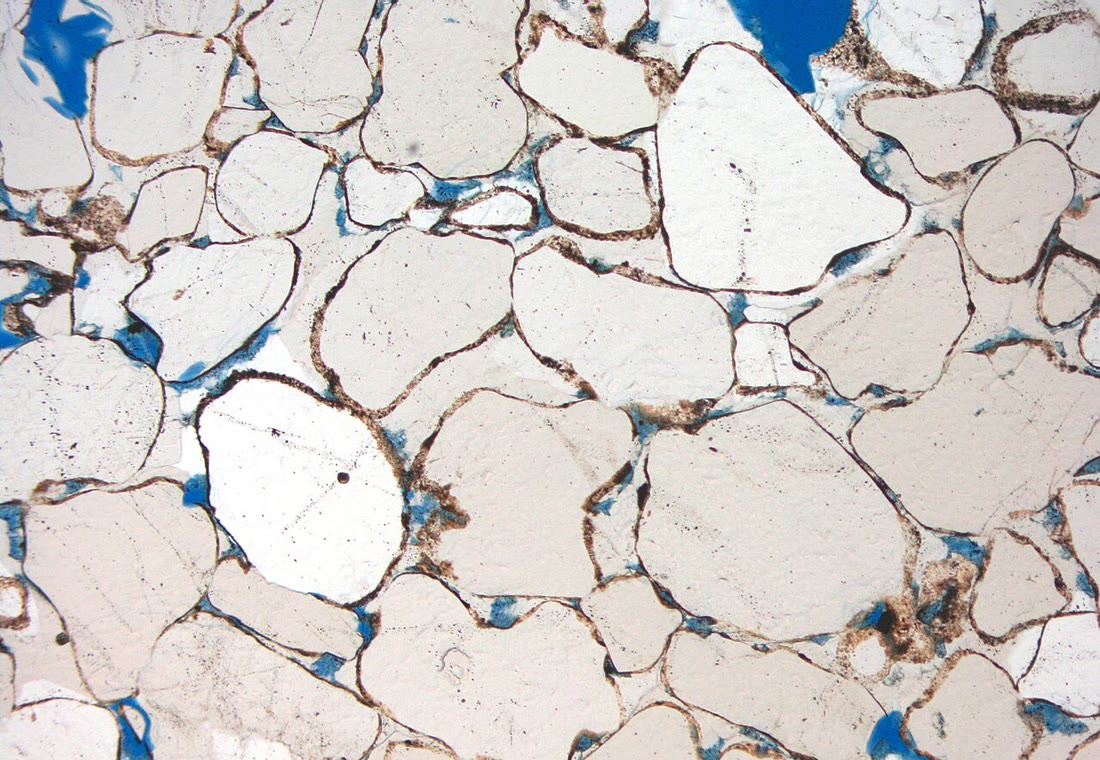
\includegraphics[width=0.62\linewidth]{images/book3/b1-quartz-overgrowths.jpg}

{\small Een dunne slijp van kwartszandsteen, het Potsdam-zandsteen (Cambrium) van de staat New York, in \omterm{def:b1:field-lab-methods-1:microscope}{vlakgepolariseerd licht}. De afgeronde klastische korrels worden begrensd door donkere randen van stof en klei; het heldere kwarts buiten de randen is \omterm{def:b1:diagenesis-basins:cement}{cement} dat op de korrels groeide, in optische continuïteit met hen, tot de naburige overgroei langs rechte vlakken samenkwam. Blauwe hars vult wat van de poriën is overgebleven. (M.~C.~Rygel, CC~BY-SA~4.0, via Wikimedia Commons; schaalbalk van het origineel bijgesneden.)}
\label{fig:b1:diagenesis-basins:overgrowths}
\end{omfigure}
% ledger: commons:potsdam

Niet elke verandering vernietigt porositeit. Water dat onderverzadigd is ten opzichte van een \omterm{def:b1:rock-forming-minerals:mineral}{mineraal} lost het op: korrels van \omterm{def:b1:rock-forming-minerals:groups}{veldspaat} en van carbonaat, en eerder carbonaatcement, kunnen worden verwijderd en een secundaire porositeit achterlaten, poriën gevormd als de korrels die zij vervangen. Kleimineralen groeien op hun beurt in de poriën, als bekleding op de korrels of als kristallen die de poriën vullen en de doorgangen ertussen vernauwen, zodat de permeabiliteit daalt. Ook de mineralen van het sediment veranderen: het aragoniet van schelpen en van de \omterm{def:b1:chemical-biogenic-sediments:factory}{carbonaatfabriek} keert terug naar calciet, dat stabiel is aan het oppervlak, en calciet kan in aanwezigheid van magnesiumhoudend water dolomiet worden.
% ledger: og:diagenesis

De vervanging van calciet door dolomiet, dolomitisatie, is een reactie met
magnesium uit het water,
\[
  \ce{2 CaCO3 + Mg^2+ -> CaMg(CO3)2 + Ca^2+},
\]
en zij verandert het volume van de vaste stof.

\begin{proposition}[Dolomitisatie creëert porositeit]\label{prop:b1:diagenesis-basins:dolomite}
Als twee mol calciet met dichtheid $\rho_c$ worden vervangen door één mol dolomiet met dichtheid $\rho_d$, neemt het volume van de vaste stof af met de fractie
\[
  1 - \frac{M_d/\rho_d}{2M_c/\rho_c},
\]
waarin $M_c$ en $M_d$ de molaire massa's zijn. Met $\rho_c = \qty{2.71}{g.cm^{-3}}$
en $\rho_d = \qty{2.84}{g.cm^{-3}}$ bedraagt deze fractie \qty{12.1}{\percent}.
\end{proposition}

\begin{proof}
Het molaire volume van een \omterm{def:b1:rock-forming-minerals:mineral}{mineraal} is zijn molaire massa gedeeld door zijn dichtheid. Twee mol calciet nemen $2M_c/\rho_c$ in beslag en één mol dolomiet $M_d/\rho_d$; het verloren deel is één min hun verhouding. Met $M_c = \qty{100.09}{g.mol^{-1}}$ en $M_d = \qty{184.40}{g.mol^{-1}}$ zijn de twee volumes $2\times\qty{36.93}{cm^3} = \qty{73.86}{cm^3}$ en \qty{64.93}{cm^3}, en $1 - 64.93/73.86 = \num{0.121}$.
\end{proof}

Als het buitenvolume van het gesteente niet verandert, is de verloren vaste stof poriënruimte die erbij komt: een kalksteen met porositeit \num{0.10} die mol voor mol door dolomiet is vervangen, heeft een porositeit van ongeveer \num{0.21}. De reactie heeft veel magnesium nodig, dat zeewater op ongeveer \qty{1.28}{g} per kilogram bevat; zij wordt bevorderd waar pekels of zeewater lang door het gesteente stromen (\cref{exo:b1:diagenesis-basins:12}).
% ledger: hom:calcite, webmineral:others, teos10:reference-composition, teos10:reference-salinity

\omterm{def:b1:diagenesis-basins:diagenesis}{Diagenese} volgt de geschiedenis van het sediment. Vlak na de afzetting, nabij het oppervlak, is het poriënwater nog dat van de zee, het meer of de regen: sedimenten zijn doorgraven, vroeg gecementeerd op de zeebodem of in de bodem, en aragoniet verandert in calciet. Met begraving en verhitting domineren \omterm{def:b1:diagenesis-basins:compaction}{compactie}, drukoplossing en kwartscementatie. Als het bekken later wordt opgeheven en geërodeerd, stroomt zoet water van het oppervlak terug in de gesteenten en lost opnieuw carbonaat en \omterm{def:b1:rock-forming-minerals:groups}{veldspaat} op. Een dunne slijp legt de volgorde van deze gebeurtenissen vast: een \omterm{def:b1:diagenesis-basins:cement}{cement} dat de porie vult die een opgeloste korrel heeft achtergelaten, is jonger dan de oplossing, en een overgroei die door \omterm{def:b1:diagenesis-basins:compaction}{compactie} is gebroken, is ouder dan de \omterm{def:b1:diagenesis-basins:compaction}{compactie}.

\section{Sedimentaire bekkens}\label{sec:b1:diagenesis-basins:basins}

Sediment van kilometers dik hoopt zich alleen op waar de vloer blijft zinken.

\begin{definition}[Sedimentair bekken]\label{def:b1:diagenesis-basins:basin}
Een \emph{sedimentair bekken}\index{sedimentair bekken} is een gebied van het aardoppervlak waar de \omterm{def:b1:layered-earth:layers}{korst} gedurende lange tijd is gesubsideerd, enkele miljoenen tot enkele honderden miljoenen jaren, en waar de zo gecreëerde ruimte is gevuld met sediment, honderden meters tot vele kilometers dik.
\end{definition}

\begin{definition}[Subsidentie, tektonische subsidentie]\label{def:b1:diagenesis-basins:subsidence}
De \emph{subsidentie}\index{subsidentie} van een bekken is de neerwaartse beweging van zijn basement, het oppervlak waarop zijn sedimenten rusten, gemeten ten opzichte van een vast referentiepunt zoals het middelpunt van de aarde. Zijn \emph{tektonische
subsidentie}\index{tektonische subsidentie} is het deel dat te wijten is aan de processen die het bekken maken, te onderscheiden van het extra zinken door het gewicht van het sediment en het water dat het vult; zij wordt gemeten aan de subsidentie die het basement alleen onder water zou hebben gehad.
\end{definition}

Wat de vloer doet zinken is de ligging van het bekken in de plaat (figuur hieronder).

\begin{description}
  \item[Riftbekkens.] Normale breuken rekken de \omterm{def:b1:layered-earth:layers}{korst}, en blokken zakken ertussen (\cref{ch:b1:rifts-ridges-margins}). De bekkens zijn smal en asymmetrisch, halve grabens die het snelst worden gevuld tegen hun begrenzende breuk. De olievelden van de Noordzee liggen in de structuren van haar Viking- en Centrale Graven, begraven onder jongere sedimenten. Wanneer het rekken stopt, koelt de verdunde en verhitte \omterm{def:b1:layered-earth:lithosphere}{lithosfeer} af, krimpt en blijft zij, langzaam, gedurende tientallen miljoenen jaren zinken. De centrale Noordzee, waarvan de laatste grote rekking eindigde in het midden van het Krijt, zakte toen als een brede, schotelvormige bekken, achtereenvolgens gevuld met krijt, zandsteen en, gedurende het grootste deel van het Tertiair, schalie en kleisteen; haar basement, alleen door water belast, zou in het midden \qtyrange{1100}{1400}{m} zijn gezakt.
  \item[Passieve marges.] Waar de rift een oceaan werd, maakt dezelfde afkoeling dat elke marge na het uiteenvallen zakt, en een wig van sediment die naar de oceaan toe dikker wordt bouwt zich op over de oude riftbekkens.
  \item[Voorlandbekkens.] Vóór een overschuivingsgordel buigt het gewicht van de opeengestapelde overschuivingsschubben de \omterm{def:b1:layered-earth:lithosphere}{lithosfeer} naar beneden, door \omterm{def:b1:isostasy-gravity:isostasy}{isostasie}, tot een bekken dat het diepst is tegen de gordel en wordt gevuld met het puin dat eruit is geërodeerd. Het meeste van de Krijtgesteenten van westelijk Canada werd in zo'n bekken afgezet, vóór de Rocky Mountains.
  \item[Intracratonische bekkens.] In het binnenland van oude continenten, ver van elke plaatgrens, zijn brede ronde of ovale gebieden gedurende zeer lange tijden langzaam gezonken. Het Parijse bekken is het centrum van zo'n structurele depressie, tussen de oude massieven van Bretagne, het Centraal Massief en de Vogezen en Ardennen.
  \item[Bekkens bij horizontale verschuiving.] Waar een breuk met horizontale verschuiving zijdelings uitwijkt in de zin die de wanden uiteentrekt --- een ontlastende bocht --- zakt een parallellogram van \omterm{def:b1:layered-earth:layers}{korst} tussen de twee breukstrengen: een trekbekken, zoals die van de regio van Los Angeles langs het San-Andreassysteem.
\end{description}
% ledger: ws:basins, sc80:north-sea, britannica:paris-basin

Waarom de \omterm{def:b1:layered-earth:lithosphere}{lithosfeer} in elke situatie zinkt, met welke snelheid, en hoe de bekkens zich tot elkaar verhouden, is het onderwerp van Boek~4; hier worden zij onderscheiden naar waar zij liggen en naar de vorm van hun vulling.

\begin{omfigure}
\begin{tikzpicture}[font=\scriptsize, line join=round]
% (a) rift: a half-graben
\begin{scope}
  \fill[lith granite] (0,0) -- (0,1.6) -- (1.4,1.6) -- (2.2,0.2) -- (5.0,1.0) -- (5.0,0) -- cycle;
  \fill[lith shale] (1.4,1.6) -- (2.2,0.2) -- (5.0,1.0) -- (5.0,1.6) -- cycle;
  \fill[lith sandstone] (1.4,1.6) -- (1.75,0.99) -- (5.0,1.25) -- (5.0,1.6) -- cycle;
  \draw[normal fault, thick] (1.4,1.6) -- (2.3,0.0);
  \draw[black!70] (0,1.6) -- (5.0,1.6);
  \node[anchor=south west] at (0,1.65) {(a) rift: een halve graben};
  \node[fill=white, fill opacity=0.8, text opacity=1, inner sep=1pt] at (3.9,0.3) {basement};
  \node[fill=white, fill opacity=0.8, text opacity=1, inner sep=1pt] at (0.65,0.8) {voetwand};
\end{scope}
% (b) passive margin: a seaward-thickening wedge over thinned crust
\begin{scope}[xshift=6.6cm]
  \fill[lith sea] (2.0,1.6) -- (5.0,1.6) -- (5.0,0.75) -- (3.6,0.95) -- cycle;
  \fill[lith granite] (0,0) -- (0,1.2) -- (2.0,1.0) -- (3.6,0.35) -- (5.0,0.05) -- (5.0,0) -- cycle;
  \fill[lith shale] (0,1.2) -- (2.0,1.0) -- (3.6,0.35) -- (5.0,0.05) -- (5.0,0.75) -- (3.6,0.95) -- (2.0,1.6) -- (0,1.6) -- cycle;
  \draw[black!70] (0,1.6) -- (2.0,1.6) -- (3.6,0.95) -- (5.0,0.75);
  \draw[blue!60!black, thick] (2.0,1.6) -- (5.0,1.6);
  \node[anchor=south west] at (0,1.65) {(b) passieve marge};
  \node[fill=white, fill opacity=0.8, text opacity=1, inner sep=1pt] at (1.0,0.45) {verdunde continentale korst};
  \node[anchor=north east] at (5.0,1.58) {oceaan};
\end{scope}
% (c) foreland basin: asymmetric, deepest against the thrust belt
\begin{scope}[yshift=-3.3cm]
  \fill[lith granite] (0,0) -- (0,0.55) -- (5.0,1.35) -- (5.0,0) -- cycle;
  \fill[lith sandstone] (0,0.55) -- (5.0,1.35) -- (5.0,1.6) -- (0,1.6) -- cycle;
  \fill[lith conglomerate] (1.0,1.6) -- (3.6,1.6) -- (1.0,1.0) -- cycle;
  \fill[omLithSchist, draw=black!70] (0,0.95) -- (1.9,1.6) -- (1.3,1.95) -- (0.4,2.25) -- (0,2.3) -- cycle;
  \draw[thrust fault] (0,0.95) -- (1.9,1.6);
  \draw[thrust fault] (0,1.55) -- (1.15,1.95);
  \draw[black!70] (1.9,1.6) -- (5.0,1.6);
  \node[anchor=south west] at (2.0,1.65) {(c) voorlandbekken};
  \node[anchor=south west, inner sep=1pt] at (0.25,2.3) {overschuivingsgordel};
  \node[fill=white, fill opacity=0.8, text opacity=1, inner sep=1pt] at (3.9,0.35) {basement};
\end{scope}
% (d) intracratonic basin: a broad sag, layers thickening to the centre
\begin{scope}[xshift=6.6cm, yshift=-3.3cm]
  \fill[lith granite] (0,0) -- (0,1.5) .. controls (1.6,1.1) and (2.0,0.3) .. (2.5,0.3) .. controls (3.0,0.3) and (3.4,1.1) .. (5.0,1.5) -- (5.0,0) -- cycle;
  \fill[lith limestone] (0,1.5) .. controls (1.6,1.1) and (2.0,0.3) .. (2.5,0.3) .. controls (3.0,0.3) and (3.4,1.1) .. (5.0,1.5) -- (5.0,1.6) -- (0,1.6) -- cycle;
  \fill[lith shale] (0.6,1.6) .. controls (1.6,1.35) and (2.1,0.85) .. (2.5,0.85) .. controls (2.9,0.85) and (3.4,1.35) .. (4.4,1.6) -- cycle;
  \fill[lith sandstone] (1.3,1.6) .. controls (1.9,1.5) and (2.2,1.3) .. (2.5,1.3) .. controls (2.8,1.3) and (3.1,1.5) .. (3.7,1.6) -- cycle;
  \draw[black!70] (0,1.6) -- (5.0,1.6);
  \node[anchor=south west] at (0,1.65) {(d) intracratonisch bekken};
  \node[fill=white, fill opacity=0.8, text opacity=1, inner sep=1pt] at (4.2,0.4) {basement};
\end{scope}
\end{tikzpicture}

{\small Vier soorten \omterm{def:b1:diagenesis-basins:basin}{sedimentair bekken} in doorsnede (schematisch, niet op schaal; verticale schaal overdreven). (a)~Een rift: de vulling wordt dikker tegen de begrenzende breuk van een halve graben. (b)~Een passieve marge: een wig van sediment die naar de oceaan toe dikker wordt over verdunde continentale \omterm{def:b1:layered-earth:layers}{korst}. (c)~Een voorlandbekken, het diepst tegen de overschuivingsgordel waarvan het gewicht het naar beneden buigt, en gevoed door zijn puin, het grofst (conglomeraat) nabij de gordel; de gordel schuift over de rand van zijn eigen bekken heen. (d)~Een intracratonisch bekken: een brede zakking waarvan de lagen naar het centrum toe dikker worden.}
\label{fig:b1:diagenesis-basins:types}
\end{omfigure}

\begin{inthefield}[Hoe bekkens bekend zijn]
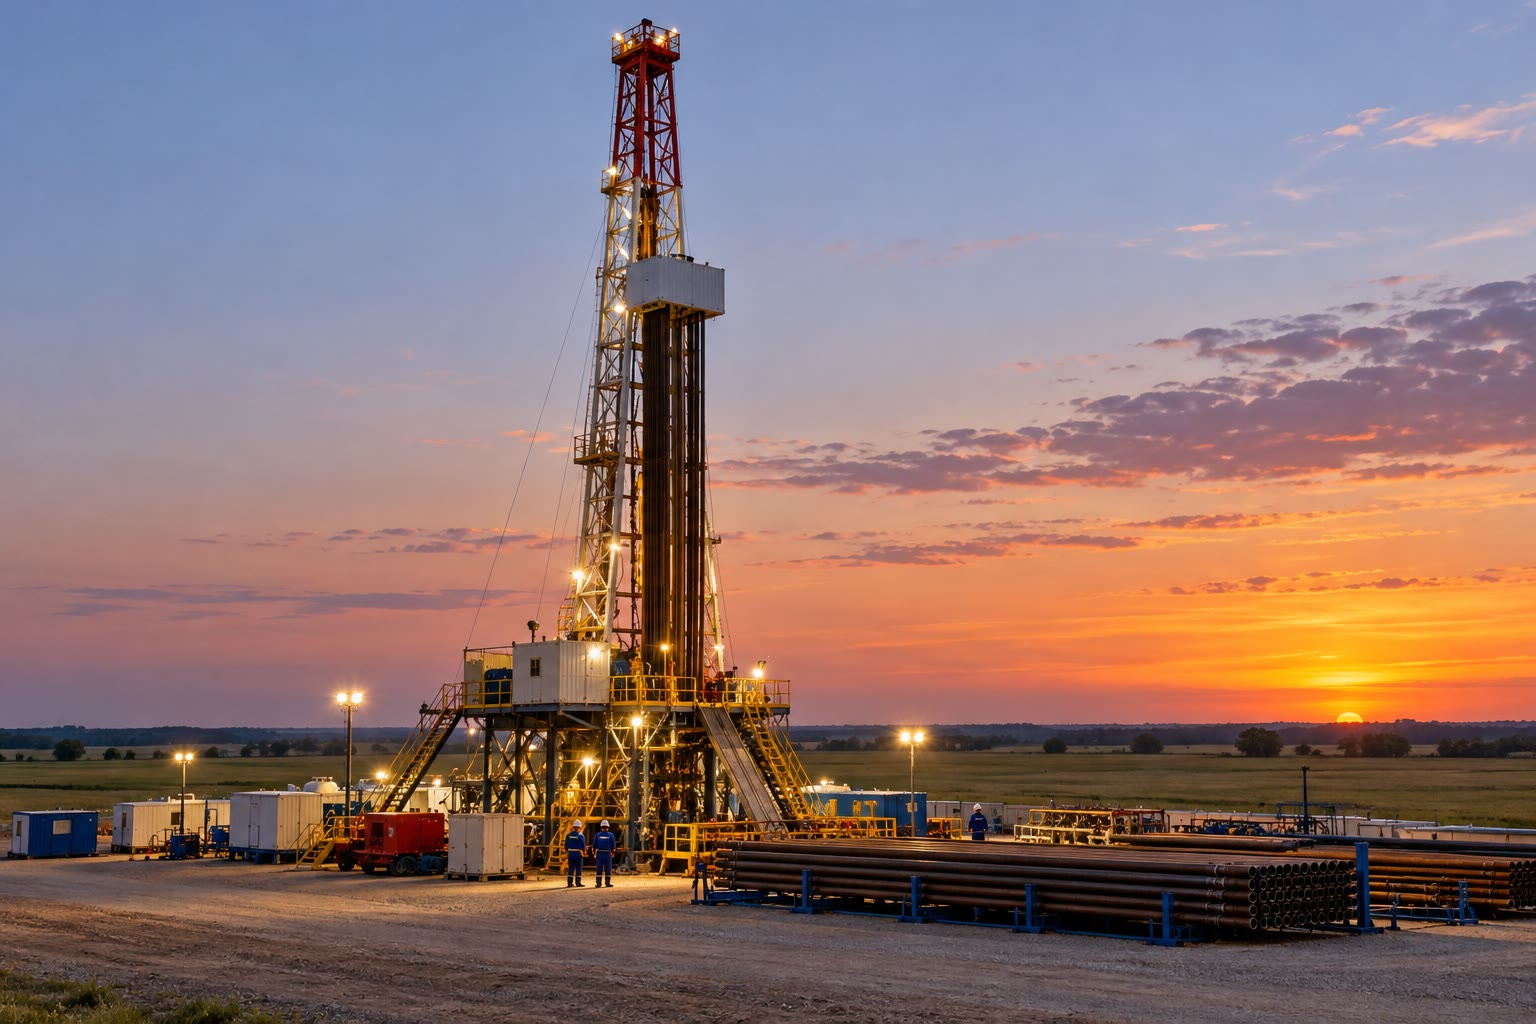
\includegraphics[width=0.3\linewidth]{images/book3/ai/b1-drilling-rig.jpg}\hfill
\begin{minipage}[b]{0.67\linewidth}
Bijna alles wat over de diepe vulling van een bekken bekend is, komt uit de zoektocht naar olie, gas en water. Seismische reflectie-onderzoeken brengen zijn lagen en zijn breuken over duizenden vierkante kilometers in beeld; putten bemonsteren het op één punt. Een put levert de gesteentesplinters die de boor afsnijdt, op intervallen kernen, en doorlopende logs van de fysische eigenschappen van de gesteenten rond het boorgat, waaruit de porositeit meter voor meter wordt afgelezen. De porositeit--diepte-curven van de \omterm{prop:b1:diagenesis-basins:athy}{wet van Athy}, en de subsidentiegeschiedenissen van bekkens, zijn voor het eerst uit zulke putten opgebouwd.
\end{minipage}

\smallskip
{\small Een landboorinstallatie bij schemering, met buizen opgestapeld op rekken op de voorgrond (AI-illustratie).}
\end{inthefield}
% ledger: sc80:north-sea

\section{Subsidentie, accommodatie en zeeniveau}\label{sec:b1:diagenesis-basins:accommodation}

Sediment kan zich alleen opstapelen waar er ruimte voor is onder het niveau waarop het verder zou worden verplaatst. In de zee ligt dat niveau dicht bij het zeeniveau, en de ruimte is een kwestie van twee bewegingen: die van de vloer, en die van het zeeoppervlak.

\begin{definition}[Accommodatie]\label{def:b1:diagenesis-basins:accommodation}
De \emph{accommodatie}\index{accommodatie} op een punt van een bekken is de ruimte die beschikbaar is voor sediment om zich daar op te hopen: de verticale afstand van de top van het sediment tot het zeeniveau, het basisniveau van de mariene afzetting. De accommodatie die in een tijdsinterval wordt gecreëerd, is de toename van de afstand van een referentievlak dat aan het basement is verbonden tot het zeeniveau.
\end{definition}

\begin{definition}[Eustasie, relatief zeeniveau]\label{def:b1:diagenesis-basins:eustasy}
\emph{Eustasie}\index{eustasie} is de verandering van het niveau van de wereldoceaan, gemeten ten opzichte van een vast referentiepunt, het middelpunt van de aarde, veroorzaakt door een verandering van het watervolume in de oceaan of van het volume van de oceaanbekkens; zij is overal dezelfde. Het \emph{relatief
zeeniveau}\index{relatief zeeniveau} op een plaats is de hoogte van het zeeoppervlak boven een daar aan het basement verbonden referentievlak; het verandert door eustasie en door de verticale beweging van de grond.
\end{definition}

\begin{proposition}[Het accommodatiebudget]\label{prop:b1:diagenesis-basins:budget}
In een tijdsinterval zij $\Delta E$ de eustatische stijging van het zeeniveau en $S$ de \omterm{def:b1:diagenesis-basins:subsidence}{subsidentie} van het basement (beide positief omhoog voor de zee, omlaag voor de vloer). De gecreëerde \omterm{def:b1:diagenesis-basins:accommodation}{accommodatie} is
\[
  \Delta A = \Delta E + S ,
\]
en zij wordt gedeeld tussen de dikte van het sediment dat boven het referentievlak wordt toegevoegd, $\Delta T$, en de verdieping van het water, $\Delta W$:
$\Delta E + S = \Delta T + \Delta W$.
\end{proposition}

\begin{proof}
Meet hoogten vanaf het vaste referentiepunt. Zij $e$ de hoogte van het zeeoppervlak,
$b$ die van het referentievlak, $T$ de dikte van het sediment boven het referentievlak,
en $W$ de diepte van het water boven het sediment, zodat $e = b + T + W$. Het
\omterm{def:b1:diagenesis-basins:eustasy}{relatief zeeniveau} is $R = e - b = T + W$. Over het interval geldt $\Delta e =
\Delta E$ en $\Delta b = -S$, dus $\Delta R = \Delta E + S$; en $\Delta R =
\Delta T + \Delta W$.
\end{proof}

Een zeebodem die op een constante diepte blijft ($\Delta W = 0$) wordt precies even snel gevuld als er \omterm{def:b1:diagenesis-basins:accommodation}{accommodatie} ontstaat; een die ondieper wordt, wordt sneller gevuld, en de kustlijn schuift naar zee; een die dieper wordt, wordt uitgehongerd. $\Delta T$ is de verandering van de dikte van de hele stapel boven het referentievlak: zij telt het nieuwe sediment dat is afgezet, minus het dunner worden van de oudere sedimenten eronder terwijl zij compacteren, zodat \omterm{def:b1:diagenesis-basins:compaction}{compactie} zelf ruimte maakt voor meer sediment (figuur hieronder).

\begin{omfigure}
\begin{tikzpicture}[font=\footnotesize, >=Stealth]
\def\col#1#2#3#4#5{% x, datum, sediment top, sea, label
  \fill[lith granite] (#1,0.2) rectangle ++(1.4,#2-0.2);
  \fill[lith shale] (#1,#2) rectangle ++(1.4,#3-#2);
  \fill[lith sea] (#1,#3) rectangle ++(1.4,#4-#3);
  \draw[black!70] (#1,#2) -- ++(1.4,0);
  \draw[blue!60!black, thick] (#1-0.2,#4) -- ++(1.8,0);
  \node[anchor=north] at (#1+0.7,0.15) {#5};}
\draw[black!60, dash dot] (-0.6,0.9) -- (8.6,0.9) node[anchor=west, align=left] {vast\\ referentiepunt};
\col{0}{1.5}{3.0}{3.6}{tijd $t_1$}
\col{4.4}{1.0}{3.4}{3.9}{tijd $t_2$}
% eustasy
\draw[<->, omThm] (3.0,0.9) -- (3.0,3.6) node[midway, fill=white, inner sep=1pt] {$e_1$};
\draw[<->, omThm] (7.4,0.9) -- (7.4,3.9) node[midway, fill=white, inner sep=1pt] {$e_2$};
% subsidence of the datum
\draw[dashed, black!60] (1.4,1.5) -- (4.4,1.5);
\draw[->, thick] (4.2,1.5) -- (4.2,1.0) node[midway, anchor=east] {$S$};
% relative sea level
\draw[<->] (-0.35,1.5) -- (-0.35,3.6) node[midway, anchor=east] {$R_1$};
\draw[<->] (6.05,1.0) -- (6.05,3.9) node[midway, anchor=west] {$R_2$};
\node[anchor=west] at (1.5,2.25) {$T_1$};
\node[anchor=west] at (1.5,3.3) {$W_1$};
\node at (5.1,2.2) {$T_2$};
\node at (5.1,3.65) {$W_2$};
\node[anchor=south, align=center, blue!60!black] at (5.1,3.95) {zeeniveau};
\node[anchor=west, align=left, font=\scriptsize] at (8.6,2.4) {$R = e - b = T + W$\\[2pt] $\Delta R = \Delta E + S$\\ $\phantom{\Delta R} = \Delta T + \Delta W$};
\end{tikzpicture}

{\small \omterm{def:b1:diagenesis-basins:accommodation}{Accommodatie} op één plaats op twee tijdstippen (schematisch). Tussen $t_1$ en
$t_2$ stijgt het zeeniveau met $\Delta E = e_2 - e_1$ boven het vaste referentiepunt en zakt het basement met $S$: het \omterm{def:b1:diagenesis-basins:eustasy}{relatief zeeniveau} $R$ groeit met $\Delta E + S$, de gecreëerde \omterm{def:b1:diagenesis-basins:accommodation}{accommodatie}, die wordt verdeeld over meer sediment ($T_2 > T_1$) en een verandering van de waterdiepte (hier een lichte ondiepte, $W_2 < W_1$).}
\label{fig:b1:diagenesis-basins:accommodation}
\end{omfigure}

Een bekken zinkt niet alleen door zijn \omterm{def:b1:diagenesis-basins:subsidence}{tektonische subsidentie}: het sediment dat het vult is een belasting, en de \omterm{def:b1:layered-earth:lithosphere}{lithosfeer} zakt daaronder verder.

\begin{proposition}[Sedimentbelasting versterkt subsidentie]\label{prop:b1:diagenesis-basins:loading}
In lokale (Airy-)\omterm{def:b1:isostasy-gravity:isostasy}{isostasie} boven een \omterm{def:b1:layered-earth:layers}{mantel} van dichtheid $\rho_m$ bevat een bekken waarvan het basement, alleen door water van dichtheid $\rho_w$ belast, op de diepte $Y$ onder het zeeniveau zou liggen, wanneer het tot zeeniveau is gevuld met sediment van gemiddelde dichtheid $\rho_s$, de dikte
\[
  h = Y\,\frac{\rho_m - \rho_w}{\rho_m - \rho_s}
\]
van sediment. Op het land, gevuld tot het niveau van de omgeving met lucht erboven, is de factor $\rho_m/(\rho_m - \rho_s)$.
\end{proposition}

\begin{proof}
Vergelijk de twee kolommen met dezelfde \omterm{def:b1:layered-earth:lithosphere}{lithosfeer}, van massa $M$ per oppervlakte-eenheid en dikte $L$, tot een \omterm{def:b1:isostasy-gravity:isostasy}{compensatiediepte} $z_c$ onder beide. De met water belaste kolom bevat $\rho_w Y + M + \rho_m(z_c - Y - L)$; de met sediment gevulde $\rho_s h + M + \rho_m(z_c - h - L)$. Volgens \cref{prop:b1:isostasy-gravity:equal-mass} zijn de twee massa's gelijk, dus
$\rho_w Y - \rho_m Y = \rho_s h - \rho_m h$, dat is $h(\rho_m - \rho_s) =
Y(\rho_m - \rho_w)$. Met lucht in plaats van water wordt $\rho_w$ door nul vervangen.
\end{proof}

Met $\rho_m = \qty{3300}{kg.m^{-3}}$, $\rho_w = \qty{1030}{kg.m^{-3}}$ en sediment van gemiddelde dichtheid \qty{2300}{kg.m^{-3}} is de factor
$2270/1000 = \num{2.27}$: een bekken waarvan de \omterm{def:b1:diagenesis-basins:subsidence}{tektonische subsidentie} ruimte zou maken voor \qty{1}{km} water, bevat \qty{2.27}{km} sediment. Op het land zou de factor $3300/1000 = \num{3.3}$ zijn. De dichtheid van de vulling is niet constant: zij neemt toe naarmate het sediment compacteert, en de factor met haar, zodat het omzetten van een sedimentdikte in een \omterm{def:b1:diagenesis-basins:subsidence}{tektonische subsidentie} de \omterm{def:b1:diagenesis-basins:compaction}{decompactie} van elke laag vereist, tijdstap voor tijdstap. Die procedure, backstripping, hoort bij Boek~4.

Het zeeniveau zelf is verre van vast. Tijdens het Laatste Glaciaal Maximum bedekten ijskappen een groot deel van Noord-Amerika en Noord-Europa, en het water dat in hen was opgesloten, was aan de oceaan onttrokken. Gecorrigeerd voor de reactie van de vaste aarde op de veranderende belastingen van ijs en water, geven de waarnemingen van vroegere kustlijnen een zeeniveau dat snel daalde met ongeveer \qty{40}{m} ongeveer \num{30000} jaar geleden en daarna langzaam tot \qty{134}{m} onder dat van vandaag, tussen \qtyrange{29}{21}{\ka}; het geaarde ijs bevatte toen ongeveer \qty{52e6}{km^3} meer dan vandaag. De vaak genoemde waarde van \qty{125}{m} is kleiner omdat zij meestal niet voor deze isostatische effecten is gecorrigeerd. De ontijzing kwam vooral tussen ongeveer \qty{16.5}{\ka} en \qty{8.2}{\ka}, gemiddeld \qty{12}{m} per duizend jaar, en met \qty{40}{mm} per jaar of meer tussen \qty{14.5}{\ka} en \qty{14.0}{\ka}.
% ledger: lambeck:lgm, lambeck:deglaciation

Oudere laagstanden worden afgelezen aan de zuurstofisotopen van foraminiferen in diepzeekernen, die het volume van ijs op het land registreren. Het stapelen van vijf van zulke reconstructies over de laatste \num{800000} jaar, en van zeven over de laatste \num{430000}, middelt de fouten van elk uit; geschaald op het Holoceen en op de laatste glaciale laagstand draagt de stapel een onzekerheid van \qtyrange{9}{12}{m} (figuur hieronder). Hij toont de glaciale cycli als een zaagtand: langzame dalingen van het zeeniveau, elk beëindigd door een snelle stijging --- vijfmaal in de laatste \num{800000} jaar een stijging van meer dan \qty{100}{m} in minder dan \num{20000} jaar. \omterm{def:b1:diagenesis-basins:eustasy}{Eustasie} op deze schaal verschuift de kustlijn heen en weer over de continentale plateaus.
% ledger: spratt:stack, data:b3-sealevel-stack

\begin{omfigure}
\begin{tikzpicture}[font=\footnotesize]
\begin{axis}[width=16cm, height=4.8cm, xmin=0, xmax=800, ymin=-150, ymax=40,
    x dir=reverse, xlabel={leeftijd (duizenden jaren geleden)}, xlabel style={yshift=2pt},
    ylabel={zeeniveau (m)}, ytick={-150,-100,-50,0},
    title={(a) de laatste \num{800000} jaar (vijf reeksen)}, title style={font=\footnotesize},
    axis on top]
  \addplot[draw=none, name path=hi] table[x=age, y=hi] {figdata/out/bachelor-1-sea_level-long.dat};
  \addplot[draw=none, name path=lo] table[x=age, y=lo] {figdata/out/bachelor-1-sea_level-long.dat};
  \addplot[omThm!25] fill between[of=hi and lo];
  \addplot[thin, omThm] table[x=age, y=sl] {figdata/out/bachelor-1-sea_level-long.dat};
  \draw[black!50, densely dotted] (axis cs:0,0) -- (axis cs:800,0);
\end{axis}
\end{tikzpicture}

\medskip
\begin{tikzpicture}[font=\footnotesize]
\begin{axis}[width=16cm, height=4.8cm,
    xmin=0, xmax=140, ymin=-160, ymax=40, x dir=reverse,
    xlabel={leeftijd (duizenden jaren geleden)}, ylabel={zeeniveau (m)},
    ytick={-150,-100,-50,0},
    title={(b) de laatste \num{140000} jaar (zeven reeksen)}, title style={font=\footnotesize},
    axis on top]
  \addplot[draw=none, name path=hi] table[x=age, y=hi] {figdata/out/bachelor-1-sea_level-short.dat};
  \addplot[draw=none, name path=lo] table[x=age, y=lo] {figdata/out/bachelor-1-sea_level-short.dat};
  \addplot[omThm!25] fill between[of=hi and lo];
  \addplot[thick, omThm] table[x=age, y=sl] {figdata/out/bachelor-1-sea_level-short.dat};
  \draw[black!50, densely dotted] (axis cs:0,0) -- (axis cs:140,0);
  \addplot[only marks, mark=*, mark size=1.6pt, black] coordinates {(21,-134)};
  \draw[black!60, thin] (axis cs:21,-131) -- (axis cs:21,-46);
  \node[anchor=south, font=\scriptsize, fill=white, inner sep=1pt] at (axis cs:36,-46) {\qty{-134}{m} op \qty{21}{\ka} uit kustlijnen (Lambeck et al.\ 2014)};
\end{axis}
\end{tikzpicture}
{\small Mondiaal zeeniveau ten opzichte van vandaag uit de stapel van Spratt en Lisiecki (2016): de eerste hoofdcomponent van vijf reconstructies uit diepzeekernen over \num{800000} jaar (a) en van zeven over de laatste \num{140000} (b), met de band van één standaardafwijking. De laagste waarde van de stapel, \qty{-130}{m} op \qty{24}{\ka}, ligt binnen die band van de \qty{-134}{m} die uit oude kustlijnen is gevonden (stip); het laatste interglaciaal ligt ongeveer \qty{3}{m} boven vandaag op \qty{121}{\ka}. Gegevens: NOAA NCEI World Data Service for Paleoclimatology.}
\label{fig:b1:diagenesis-basins:sea-level}
\end{omfigure}
% computed in figdata/bachelor-1/sea_level.py; ledger: data:b3-sealevel-stack, spratt:stack, lambeck:lgm

Over het leven van een bekken zijn zulke schommelingen kort. Een glaciale daling van meer dan \qty{100}{m} in enkele tienduizenden jaren is snel en groot vergeleken met de \omterm{def:b1:diagenesis-basins:subsidence}{tektonische subsidentie}, die slechts over tientallen miljoenen jaren een kilometer of meer bereikt; maar de glaciale schommelingen blijven binnen een bereik van ongeveer \qty{150}{m}, zodat in de dikke vulling van een bekken de \omterm{def:b1:diagenesis-basins:subsidence}{subsidentie} het meeste van de ruimte maakt, en \omterm{def:b1:diagenesis-basins:eustasy}{eustasie} het ritme van zijn lagen bepaalt.
% ledger: data:b3-sealevel-stack, sc80:north-sea

\section{Oefeningen}

\begin{exercise}[$\star$]\label{exo:b1:diagenesis-basins:1}
Bereken met de parameters van \cref{tab:b1:diagenesis-basins:athy} de porositeit van zandsteen en van schalie op \qty{2000}{m}. Op welke diepte is de porositeit van elk tot de helft van haar oppervlaktewaarde gedaald?
% ledger: pybacktrack:compaction
\end{exercise}

\begin{exercise}[$\star$]\label{exo:b1:diagenesis-basins:2}
Gedurende een tijdsinterval stijgt het zeeniveau door \omterm{def:b1:diagenesis-basins:eustasy}{eustasie} met \qty{30}{m}, zakt het basement van een continentaal plat met \qty{50}{m}, en wordt \qty{60}{m} sediment toegevoegd boven een referentievlak op het basement. Bereken met \cref{prop:b1:diagenesis-basins:budget} de gecreëerde \omterm{def:b1:diagenesis-basins:accommodation}{accommodatie} en de verandering van de waterdiepte. Wordt het plat dieper of ondieper?
\end{exercise}

\begin{exercise}[$\star$]\label{exo:b1:diagenesis-basins:3}
De \omterm{def:b1:diagenesis-basins:subsidence}{tektonische subsidentie} van een bekken zou ruimte maken voor \qty{1.0}{km} water. Hoe dik is, met $\rho_m = \qty{3300}{kg.m^{-3}}$ en $\rho_w = \qty{1030}{kg.m^{-3}}$, het sediment dat het tot zeeniveau vult als de gemiddelde dichtheid \qty{2300}{kg.m^{-3}} is? En bij \qty{2500}{kg.m^{-3}}? Waarom geeft een dichtere vulling een dikkere?
\end{exercise}

\begin{exercise}[$\star$]\label{exo:b1:diagenesis-basins:4}
Calciet heeft de molaire massa \qty{100.09}{g.mol^{-1}} en de dichtheid \qty{2.71}{g.cm^{-3}}; dolomiet \qty{184.40}{g.mol^{-1}} en \qty{2.84}{g.cm^{-3}}. (a)~Bereken het molaire volume van elk. (b)~Met welke fractie verandert het volume van de vaste stof wanneer twee mol calciet één mol dolomiet worden? (c)~Een kalksteen met porositeit \num{0.10} wordt mol voor mol gedolomitiseerd zonder verandering van haar buitenvolume. Wat is haar nieuwe porositeit?
% ledger: hom:calcite, webmineral:others
\end{exercise}

\begin{exercise}[$\star\star$]\label{exo:b1:diagenesis-basins:5}
Een schalie vult de bovenste \qty{1000}{m} van een bekken. (a)~Bereken haar vaste dikte en haar gemiddelde porositeit. (b)~Zij wordt begraven tot haar top op \qty{2000}{m} ligt. Gebruik \cref{met:b1:diagenesis-basins:decompaction} met de top naar beneden in plaats van naar boven verplaatst, en bepaal haar nieuwe dikte en haar gemiddelde porositeit. (c)~Hoeveel water heeft elke vierkante meter van de schalie uitgedreven?
% ledger: pybacktrack:compaction
\end{exercise}

\begin{exercise}[$\star\star$]\label{exo:b1:diagenesis-basins:6}
Een zandsteen ligt tussen \qty{2500}{m} en \qty{2800}{m}. (a)~Bereken haar vaste dikte. (b)~Decompacteer haar tot het oppervlak met \cref{met:b1:diagenesis-basins:decompaction}, en schrijf elke Newton-stap op vanaf $b_0 = \qty{300}{m}$. (c)~Met welke factor heeft de begraving haar dunner gemaakt?
% ledger: pybacktrack:compaction
\end{exercise}

\begin{exercise}[$\star\star$]\label{exo:b1:diagenesis-basins:7}
Op het Laatste Glaciaal Maximum bevatte het geaarde ijs ongeveer \qty{52e6}{km^3} meer dan vandaag. Neem de dichtheid van ijs \qty{916.7}{kg.m^{-3}}, die van smeltwater \qty{1000}{kg.m^{-3}}, en de oppervlakte van de huidige oceaan \qty{361.84e6}{km^2}. (a)~Welke daling van het zeeniveau vertegenwoordigt dit ijs? (b)~Vergelijk met de \qty{134}{m} die uit oude kustlijnen is gevonden. (c)~Welke oceaanoppervlakte zou precies \qty{134}{m} geven, en waarom was de glaciale oceaan kleiner?
% ledger: lambeck:lgm, iapws:ice-density, charette:ocean-volume
\end{exercise}

\begin{exercise}[$\star\star$]\label{exo:b1:diagenesis-basins:8}
De zeeniveaustapel geeft \qty{-98.1}{m} op \qty{16}{\ka} en \qty{-9.1}{m} op \qty{8}{\ka}. (a)~Bereken de gemiddelde stijgingssnelheid, in meter per duizend jaar, en vergelijk die met de \qty{12}{m} per duizend jaar die uit oude kustlijnen voor de hoofdontijzing is gevonden. (b)~Tussen \qty{14.5}{\ka} en \qty{14.0}{\ka} steeg het zeeniveau met \qty{40}{mm} per jaar of meer. Hoeveel keer het gemiddelde is dat, en hoeveel steeg het zeeniveau in die vijfhonderd jaar?
% ledger: data:b3-sealevel-stack, lambeck:deglaciation
\end{exercise}

\begin{exercise}[$\star\star$]\label{exo:b1:diagenesis-basins:9}
Een continentaal plat ligt onder \qty{20}{m} water. Zijn basement zakt met \qty{50}{m} per miljoen jaar. (a)~Over twee miljoen jaar daalt het zeeniveau door \omterm{def:b1:diagenesis-basins:eustasy}{eustasie} met \qty{40}{m}, terwijl de waterdiepte gelijk blijft. Hoeveel \omterm{def:b1:diagenesis-basins:accommodation}{accommodatie} wordt gecreëerd, en hoeveel sediment wordt toegevoegd? (b)~Het zeeniveau daalt daarna met \qty{120}{m} in \num{20000} jaar, aan het begin van een ijstijd, en er wordt geen sediment toegevoegd. Hoe hoog boven het zeeniveau staat de vroegere zeebodem aan het eind?
\end{exercise}

\begin{exercise}[$\star\star\star$]\label{exo:b1:diagenesis-basins:10}
(a)~Toon aan dat een laag van dikte $h$ op de diepte $z$, dun vergeleken met de vervalslengte $\lambda$, bij herstel tot het oppervlak de dikte $h_0 \approx h\,(1 - \varphi(z))/(1 -
\varphi_0)$ heeft. (b)~Pas dit toe op \qty{10}{m} schalie op \qty{3000}{m}, en vergelijk met de exacte \omterm{def:b1:diagenesis-basins:compaction}{decompactie}, \qty{23.1}{m}. (c)~Waarom is de benadering iets te groot?
% ledger: pybacktrack:compaction
\end{exercise}

\begin{exercise}[$\star\star\star$]\label{exo:b1:diagenesis-basins:11}
Een bekken wordt tot zeeniveau gevuld met \qty{3000}{m} schalie, gecompacteerd volgens de \omterm{prop:b1:diagenesis-basins:athy}{wet van Athy}, met poriën vol water van dichtheid \qty{1030}{kg.m^{-3}}. (a)~Bereken de gemiddelde porositeit en de gemiddelde dichtheid van de vulling. (b)~Met \cref{prop:b1:diagenesis-basins:loading} en $\rho_m =
\qty{3300}{kg.m^{-3}}$, bereken de belastingsfactor en de met water belaste \omterm{def:b1:diagenesis-basins:subsidence}{subsidentie} die de vulling vertegenwoordigt. (c)~Waarom zou het nemen van de dichtheid van de korrels, \qty{2700}{kg.m^{-3}}, een veel grotere factor geven, en waarom zou dat fout zijn?
% ledger: pybacktrack:compaction
\end{exercise}

\begin{exercise}[$\star\star\star$]\label{exo:b1:diagenesis-basins:12}
Een kubieke meter kalksteen met porositeit \num{0.10} moet volledig worden gedolomitiseerd, mol voor mol. Zeewater bevat \qty{35.165}{g} zout per kilogram, waarvan de massafractie \num{0.0365} magnesium is (\qty{24.305}{g.mol^{-1}}). (a)~Hoeveel mol calciet bevat de kubus (molair volume uit \cref{exo:b1:diagenesis-basins:4})? (b)~Hoeveel mol magnesium heeft de reactie nodig? (c)~Welke massa en welk volume zeewater (\qty{1030}{kg.m^{-3}}) moet door de kubus stromen als zij al haar magnesium afstaat? (d)~Wat zegt het antwoord over waar dolomiet vormt?
% ledger: teos10:reference-composition, teos10:reference-salinity, hom:calcite
\end{exercise}

\section{Probleem: de vulling van een bekken decompacteren}

\begin{problem}[{Weekendprobleem --- hoe dik de sedimenten van een put waren toen zij werden afgezet, en
hoe de ruimte voor hen werd gemaakt}]
\label{pb:b1:diagenesis-basins:1}
% values: calc/ch23.py; the well, its units, ages and the eustatic changes are invented
Een put geboord op een kustvlakte, op zeeniveau, doorkruist drie eenheden voordat zij het basement op \qty{3200}{m} bereikt:
\begin{center}
\begin{tabular}{llll}
\hline
eenheid & lithologie & diepte vandaag (m) & tijd van afzetting \\
\hline
1 & zandsteen & 0--800     & \qtyrange{15}{0}{\Ma} \\
2 & schalie     & 800--2600  & \qtyrange{55}{15}{\Ma} \\
3 & krijt     & 2600--3200 & \qtyrange{75}{55}{\Ma} \\
\hline
\end{tabular}
\end{center}
Neem de parameters van \cref{tab:b1:diagenesis-basins:athy}, poriënwater van dichtheid \qty{1030}{kg.m^{-3}}, $g = \qty{9.81}{m.s^{-2}}$, en veronderstel dat elke eenheid gecompacteerd werd volgens de \omterm{prop:b1:diagenesis-basins:athy}{wet van Athy}, met haar water vrij om te ontsnappen, gedurende haar hele geschiedenis. Microfossielen tonen dat het water ondiep was, en even diep, aan het begin en aan het eind van elk interval.

\medskip
\noindent\textbf{Deel I --- De kolom vandaag.}
\begin{enumerate}
  \item Bereken de porositeit aan de top en aan de basis van elke eenheid.
  \item Bereken de gemiddelde porositeit van elke eenheid.
  \item Hoeveel water bevat elke eenheid onder één vierkante meter?
  \item Bereken de volumieke dichtheid van elke eenheid, verzadigd met water, en de gemiddelde
        dichtheid van de hele kolom.
  \item Bereken de litostatische en de hydrostatische druk aan de basis van de kolom, en de
        \omterm{def:b1:stress-strain-rheology:lithostatic}{effectieve spanning} daar.
  \item Op welke diepte zijn de porositeiten van zandsteen en schalie gelijk? Welke is de poreuzere
        onder die diepte?
\end{enumerate}

\noindent\textbf{Deel II --- De korrels.}
\begin{enumerate}[resume]
  \item Bereken de vaste dikte van elke eenheid.
  \item Wat is de vaste dikte van de hele kolom, en welk deel van de kolom van vandaag is water?
  \item Bereken voor elke eenheid de accumulatiesnelheid van korrels, in meter vaste stof per miljoen jaar.
  \item Welke eenheid had de snelste toevoer van korrels? De langzaamste?
\end{enumerate}

\noindent\textbf{Deel III --- De eenheden zoals zij werden afgezet.}
\begin{enumerate}[resume]
  \item Hoe dik was het zandsteen toen het werd afgezet? Waarom is geen berekening nodig?
  \item Decompacteer de schalie tot het oppervlak: hoe dik was zij op \qty{15}{\Ma}, toen haar afzetting net was geëindigd?
  \item Decompacteer het krijt tot het oppervlak: hoe dik was het op \qty{55}{\Ma}?
  \item Hoe dik was het krijt op \qty{15}{\Ma}, begraven onder de schalie van de vorige vraag?
  \item Wat was de dikte van de hele kolom boven het basement op \qty{55}{\Ma} en op \qty{15}{\Ma}?
  \item Bereken de sedimentatiesnelheid van elke eenheid uit haar dikte vandaag, en uit haar dikte bij afzetting. Welke is zinvol?
  \item Met welk deel is de schalie sinds \qty{15}{\Ma} dunner geworden?
\end{enumerate}

\noindent\textbf{Deel IV --- Ruimte maken.}
\begin{enumerate}[resume]
  \item Neem de top van het basement als referentievlak. Bereken met \cref{prop:b1:diagenesis-basins:budget} de \omterm{def:b1:diagenesis-basins:accommodation}{accommodatie} die is gecreëerd vanaf \qtyrange{75}{55}{\Ma}, vanaf \qtyrange{55}{15}{\Ma} en vanaf \qty{15}{\Ma} tot vandaag.
  \item Een eustatische kromme voor de regio geeft een zeeniveau dat \qty{60}{m} hoger ligt op \qty{55}{\Ma} dan op \qty{15}{\Ma}, en \qty{30}{m} hoger op \qty{15}{\Ma} dan vandaag (aangenomen waarden). Bereken de \omterm{def:b1:diagenesis-basins:subsidence}{subsidentie} van het basement in de laatste twee intervallen.
  \item Bereken de gemiddelde subsidentiesnelheid in elk, in meter per miljoen jaar.
  \item Welk aandeel van de \omterm{def:b1:diagenesis-basins:subsidence}{subsidentie} moest \omterm{def:b1:diagenesis-basins:eustasy}{eustasie} in elk interval aanvullen? Hielp of belemmerde \omterm{def:b1:diagenesis-basins:eustasy}{eustasie} de vulling van het bekken?
  \item Van de \omterm{def:b1:diagenesis-basins:accommodation}{accommodatie} die sinds \qty{15}{\Ma} is gevuld, hoeveel werd gemaakt door de \omterm{def:b1:diagenesis-basins:compaction}{compactie} van de schalie en het krijt eronder?
  \item Waarom kan de \omterm{def:b1:diagenesis-basins:subsidence}{subsidentie} van het basement niet worden afgelezen aan de dikte van de kolom vandaag?
  \item Hoe dik was de schalie-eenheid toen zij werd afgezet?
\end{enumerate}
\end{problem}
